\chapter{Detection simulation}\label{ch:detection-simulation}

\section{Generation of EMRI LISA response in TDI channels}\label{sec:generation-of-emri-lisa-response}
For the generation of the LISA response in the form of the TDI channels $A,E,T$ we use the python module \emph{FEW} (fast EMRI waveforms) \cite{Katz_2021,Chua_2021} introduced in \fullref{chap:emris} combined with the python module \emph{fastliseresponse} \cite{Katz_2022}. The waveform that is generated by \emph{FEW} in the SSB frame is of the form
\begin{equation}
    h(t) = h_+(t) + i h_\times(t),
\end{equation}
and is then transformed into the detector frame and processed into the LISA TDI channels $A,E,T$ by \emph{fastliseresponse} which we will then use to compute the SNR via \fullref{eq:optimal-snr-lisa} and perform the parameter estimation. Recall that we will ignore the $T$ channel.

\section{Parameter space}\label{sec:parameter-space}
In \fullref{list:emri-parameters} we have introduced the final 15 parameters (+ $\tobs$ and $\Delta t$) that we will use to generate the EMRI response of the LISA detector. The choice of parameter ranges will be mostly aligned with \cite[M1 model]{PhysRevD.95.103012}. While the setup for using an astrophysical population of EMRI events from which we can sample the events has been prepared and implemented, the evaluations have not been performed and is left for future works. In the present work we will randomly choose galaxies form the catalog from a restricted mass range and use the galaxy parameters ($\vartheta, \varphi, \dl(z_g, \rhubbletrue), \Mbh^g )$ for the generation, but more on that later. This means we will consider the following ranges for the parameters:
\begin{itemize}
    \item $\Mbh \in [10^5, 10^6] \Msol$ (catalog),
    \item $\mu = 10 \Msol$ (fixed),
    \item $\dl$ (catalog),
    \item $\vartheta$ (catalog),
    \item $\varphi$ (catalog),
    \item $a = 0.98$ (fixed),
    \item $p_0 \in [10 16]$ (random),
    \item $e_0 \in [0, 0.2]$ (random),
    \item $x_{I,0} \in [-1, 1]$ (random),
    \item $\vartheta_K \in [0, \pi]$ (random),
    \item $\varphi_K \in [0, 2\pi]$ (random),
    \item $\Phi_{\theta,0} \in [0, 2\pi]$ (random),
    \item $\Phi_{\phi,0} \in [0, 2\pi]$ (random),
    \item $\Phi_{r,0} \in [0, 2\pi]$ (random),
\end{itemize}
where $\mu$ and $a$ are consistent with the M1 model, $p_0$ is restricted by the \emph{FEW} module and the rest of the parameters are chosen randomly. To be precise, whenever we choose angles at random, this will be isotropic on the sphere. In the M1 model the $\Mbh$ range considered is $\Mbh \in [10^4, 10^7]$, but we restrict it to $\Mbh \in [10^5, 10^6]$ for the catalog, because otherwise the number of possible hosts are too computationally expensive. This at least holds for the reference model, where we don't use the information on $\Mbh$ from the measurement to further restrict the error volume. This still covers the region where most of the EMRI events are expected. Let us now turn to the parameters chosen from the random galaxy in the catalog. First and foremost by \emph{random}, we truly mean random. This will of course produce detection distributions that are not consistent with what we would expect from the astrophysical population of EMRI events but it provides a starting point to test the inference pipeline and to compare the results with and without using the $\Mbh$ information. In the galaxy catalog the sky localization angles $\vartheta, \varphi$ are provided without associated errors, so we just need to make sure that they are transformed into the same definition of angles as in the parameters space. For $\Mbh$ we have an uncertainty $\sigma_{\Mbh}$ and we will draw $\Mbh^\text{draw}$ a sample from a normal distribution $\normaldist{\Mbh}$ and use it as the simulation parameter. Here we do not need to be careful about the redshifting of the observed mass, as both the galaxy catalog - after mapping the stellar masses to $\Mbh$ via \fullref{eq:stellar-mass-bh-mass-relation} - and the EMRI waveform generation provide and use the source mass. For the luminosity distance $\dl$ we use the given redshift $z_g$ and its uncertainty $\sigma_{z_g}$ from the galaxy to again draw a true redshift $z^\text{draw}$ from a normal distribution $\normaldist{z_g}$ and use it to compute the luminosity distance $\dl^\text{draw} = \dl(z^\text{draw}, \rhubbletrue)$. Note that at this point we are allowed to use the true $\rhubbletrue$ because we are generating the EMRI signal and we know the true value of the Hubble constant because we have defined the nature of the simulation. Having chosen all parameters for the EMRI event, we need to further specify the generation parameters for the observation, i.e. the observation time $\tobs$ and the sampling rate $\Delta t$. Consistent with the LISA mission design \cite{colpi2024lisadefinitionstudyreport} , we choose $\tobs = 5\unit{yr}$ and $\Delta t = 10\unit{s}$. The time resolution of $\Delta t = 10\unit{s}$ corresponds to
\begin{equation}
    \Delta f = \frac{1}{\tobs} \approx 6 \times 10^{-9} \unit{Hz},
\end{equation}
and $f_\text{max}^\text{sampling} = \frac{1}{\Delta t} = 0.1 \unit{Hz}$ which aligns well with the sensitivity of LISA. We are now left with defining the cosmological parameters of our simulation before moving to the detection of the EMRI signals.

\section{Cosmological parameters}\label{sec:cosmological-parameters}
In \fullref{ch:cosmology} we introduced the $\lamcdm$ model that we will use throughout the thesis. The cosmological parameters are the reduced Hubble constant $\rhubble$ and the matter density $\Omega^m_0$ which defines $\Omega^\Lambda_0 = 1 - \Omega^m_0$. It is our goal to infer $\rhubble$ and we have introduced its prior in \fullref{sec:prior-distribution}. This means we will have to evaluate the posterior distribution at different values of $\rhubble$ in the interval $[0.6, 0.86]$. Generally, we have a step size of $\Delta \rhubble \le 0.01$ with higher precision around the true value $\rhubbletrue = 0.73$ which is defined in \fullref{eq:rhubble-true}. In this analysis we are only interested in the inference of $\rhubble$ so we fix $\Omega^m_0 = 0.25$ as defined in \fullref{eq:omega-matter-0}
where both $\rhubbletrue$ and $\Omega^m_0$ are consistent with \cite{10.1093/mnras/stab2741}.

\section{Detection of EMRI events}\label{sec:detection-of-emri-signals}
Given an EMRI LISA response in the form of the TDI channels $A,E$ and $T$, where $T$ corresponds to the \emph{null} channel and can therefore be neglected, we call the event a detection if the optimal SNR is above the threshold
\begin{equation}
    \label{eq:snr-threshold}
    \text{SNR}_\text{th} \equiv \varrho_\text{th} = 20.
\end{equation}
Recall the optimal SNR for LISA is defined in \fullref{eq:optimal-snr-lisa}. Because the generation time of the LISA response scales with the observation time $\tobs$ as well as with the SNR as can be seen in \fullref{fig:quick-snr-check-validation}, in the interest of computational efficiency, we introduce a first checkpoint called \emph{quick SNR check} where we compute the SNR for an observation time $\tobs = 1\unit{yr}$ and require $\text{SNR}_\text{th}^\text{quick} = 0.2 \cdot \text{SNR}_\text{th}$ to be exceeded. If this condition is met, we proceed to compute the optimal SNR for the full observation time $\tobs$ and compare it to the threshold $\text{SNR}_\text{th}$. If the full SNR is above the threshold, we consider the signal to be detected. This quick SNR check is a computationally efficient way to filter out signals that are extremely unlikely to be detected. Once we have detected a signal, we can proceed to compute the Cramér-Rao bounds on the parameters of the EMRI signal.

\begin{figure}
    \centering
    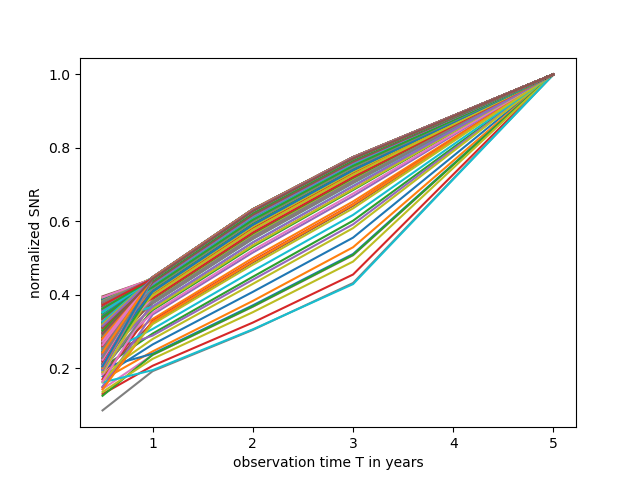
\includegraphics[width=0.49\textwidth]{SNR_observation_time.png}
    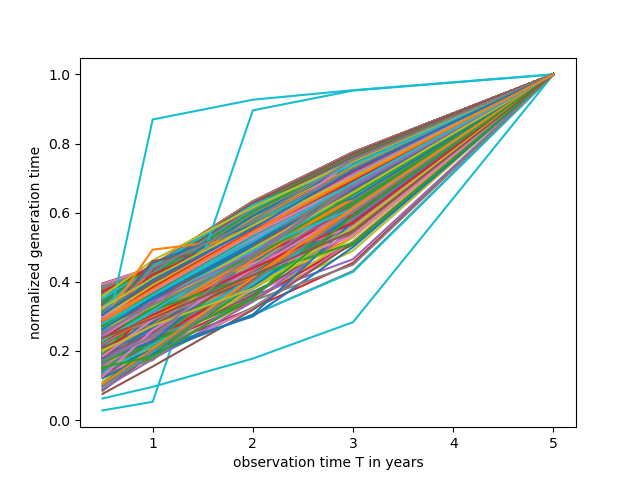
\includegraphics[width=0.49\textwidth]{generation_time_observation_time.png}
    \caption[Validation of quick SNR check]{On the left the optimal SNR as a function of observation time $\tobs$ for a large set of EMRI signals with randomly chosen parameters is shown. On the right we plot the generation time of the LISA response as a function of observation time $\tobs$ for the same set of EMRI signals. We choose a threshold of $\text{SNR}^{\text{quick}}_\text{th} = 0.2 \cdot \text{SNR}_\text{th}$ for the quick SNR check.}
    \label{fig:quick-snr-check-validation}
\end{figure}

\subsection{Computing Cramér-Rao bounds}\label{subsec:cramer-rao-bound}
As introduced in \fullref{ch:data-analyses}, the Cramér-Rao bounds $\bm{\Sigma}_\text{CR}$, i.e. lower limits for the covariance matrix, for the limit of high SNR are given by the inverse of the Fisher information matrix $\bm{\Gamma}^{-1}$. Thus, we need to compute the Fisher information matrix $\bm{\Gamma}$ (\fullref{eq:fisher-information-matrix}) for the EMRI signal, i.e. evaluate the derivatives of the waveform $\partial_{\theta^i} h(t; \theta)$ with respect to the 15 parameters $\theta$ of an EMRI event. We use the finite difference method
\begin{equation}
    \label{eq:finite-difference}
    \partial_{\theta^i} h(t; \theta) \approx \frac{h(t; \theta^i + \varepsilon) - h(t; \theta^i)}{\varepsilon},
\end{equation}
where $\varepsilon = 10^{-6}$ and $\theta$ are the simulation parameters that were used to generate the EMRI LISA response. We omitted the rest of the parameters in the notation for clarity. We can then use the derivatives to compute the components fo the Fisher information matrix via the scalar product of functions \fullref{eq:scalar-product} and store the Cramér-Rao bounds. In this fashion we create a collection of EMRI signals that were detected and for which we have computed the Cramér-Rao bounds on the parameters.

\section{Numerical bottlenecks}\label{sec:numerical-bottlenecks}
\subsection{Generation of the EMRI LISA response}\label{subsec:generation-of-the-emri-lisa-response}
For the simulation of the EMRI detections, the important consideration for the computational cost is the generation time of the waveform which is, thanks to the GPU parallelization, already very fast (see \fullref{fig:waveform-generation-time}) with an average computation time of $0.933$s. Nevertheless, this will become a bottleneck if we start using more accurate approximation when computing the derivative such as the five point stencil method that uses five evaluations of the waveform for each of the 15 parameters. This is why for now the simulation uses the finite difference method \fullref{eq:finite-difference} to compute the derivatives. [TODO: error estimation for derivatives]
\begin{figure}
    \centering
    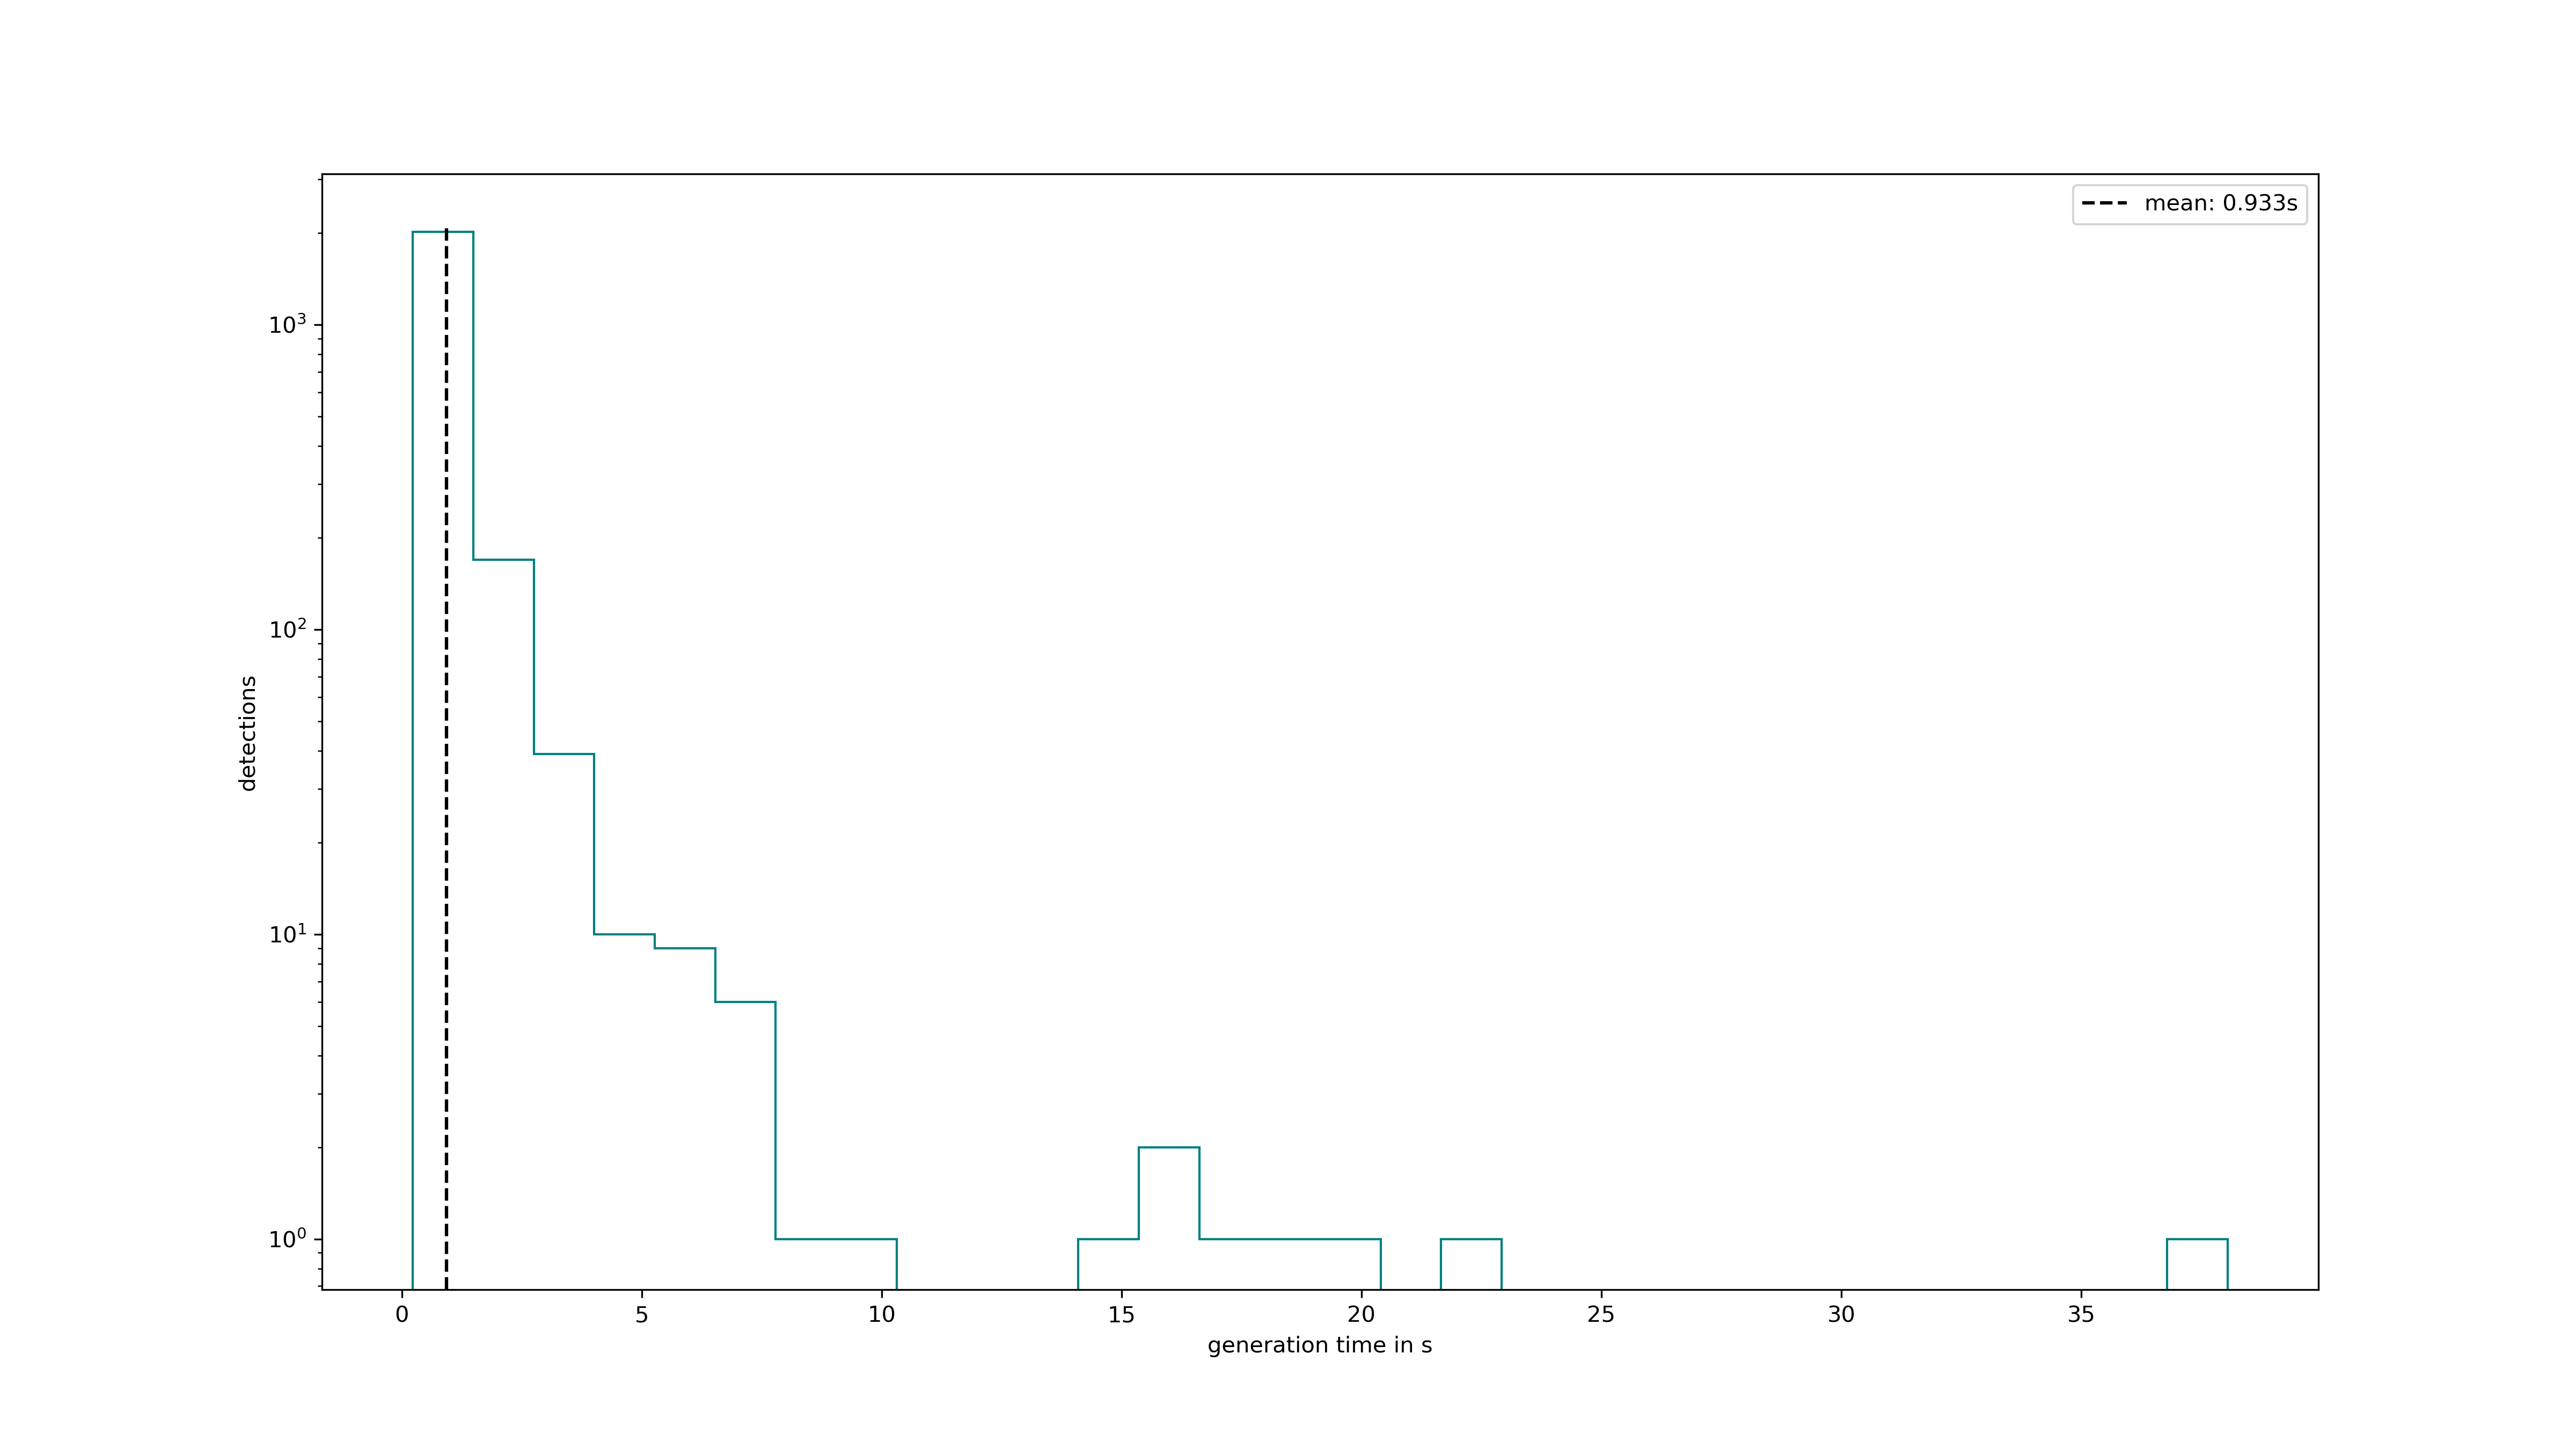
\includegraphics[width=0.8\textwidth]{generation_time.png}
    \caption[Waveform generation time histogram]{Histogram of the generation time of the EMRI LISA response using the python modules \emph{fastlisaresponse} and \emph{FEW}.}
    \label{fig:waveform-generation-time}
\end{figure}

\section{Computation of the posterior}\label{subsec:computing-the-fisher-information-matrix}
The computation of the posterior distribution has to be done for every value of $\rhubble$ in the discretized interval $[0.6, 0.86]$. For each value of $\rhubble$ we then iterate over all detections and have to compute the likelihood of each galaxy for given detection and given value of $\rhubble$. As the galaxies are weighted by the gaussian distributions in …\fullref{eq:likelihood-final}, we can reduce the sum over all galaxies in the catalog to a sum over all galaxies within an error volume defined by the detection parameter uncertainties. We use a $3 \sigma$ cutoff for the error volume, e.g. [$\hat{\varphi} - 3 \sigma_\varphi$, $\hat{\varphi} + 3 \sigma_\varphi$] for the parameter $\varphi$. Further, instead of considering the full range in redshift when integrating over $\zgw$ in \fullref{eq:likelihood-final}, we can set outer bounds $z_\text{min}, z_\text{max}$ using the prior we imposed on the range of $\rhubble$ to compute
\begin{equation}
    \label{eq:redshft-outer-bounds}
    \begin{split}
        z_\text{min} &= z(\hat{\dl} - 4\sigma_{\dl}, \rhubble_\text{min}), \\
        z_\text{max} &= z(\hat{\dl} + 4\sigma_{\dl}, \rhubble_\text{max}),
    \end{split}
\end{equation}
where $z(\dl, \rhubble)$ is the inverse of the luminosity distance function \fullref{eq:luminosity-distance-redshift-relation-lcdm}.
For the detections evaluated in \fullref{ch:galaxy-catalog-as-ground-truth} the number of possible hosts are shown in \fullref{fig:possible-hosts}. Last but not least, we take a look at the integral over $\Mbh$ in \fullref{eq:likelihood-final}. Let us first isolate the part of the integral that depends on $\Mbh$
\begin{equation}
    p(\detection |\rhubble , \galcat , \cosmologicalmodel, \backgroundinformation) \propto \int \dd \Mbh g(\Mbh) \cdot \exp \left \{ -\frac{(\hat{\Mz} - \Mbh (1 + \zgw))^2}{2 \sigma_{\Mz}^2}  \right \},
\end{equation}
where $g(\Mbh)$ are the covariance contributions and the normal distribution $\normaldist{\Mbh^{(k)}}$ terms that depend on $\Mbh$. If we compare the relative error of $\Mz$ for detections  and the galaxy catalog in \fullref{fig:relative-mass-error-distribution}, we see that the relative error is a lot smaller for the detections
\begin{equation}
    \label{eq:relative-mass-error}
    \begin{split}
        \sfrac{\sigma_{\Mz}}{\hat{\Mz}} &\le 10^{-6}, \quad \forall \detection \in \detections \\
        \sfrac{\sigma_{\Mbh}}{\Mbh} &\ge 0.2, \quad \forall \galaxy \in \galcat.
    \end{split}
\end{equation}
Hence, we can treat the exponential term effectively as a delta function and reduce the integral to
\begin{equation}
    \begin{split}
        p(\detection |\rhubble , \galcat , \cosmologicalmodel, \backgroundinformation) &\propto \int \dd \Mbh g(\Mbh) \cdot \delta (\hat{Mz} - \Mbh (1 + \zgw)) \\
        &= \frac{g(\frac{\hat{\Mz}}{1 + \zgw})}{1 + \zgw},
    \end{split}
\end{equation}
where we used to representation of the delta function
\begin{equation}
    \delta(x) = \lim_{\varepsilon \rightarrow 0} \frac{1}{\sqrt{2\pi \varepsilon}} \exp \left \{ -\frac{x^2}{2 \varepsilon} \right \}
\end{equation}
and its property
\begin{equation}
    \int \dd x g(x) \delta(f(x)) = \sum_{x_i} \frac{g(x_i)}{\abs{f'(x_i)}},
\end{equation}
where $x_i$ are the roots of $f(x) = 0$.

\section{Libraries \& deployment}\label{sec:deployment-of-the-simulation}
Both the simulation of EMRI events and the computation of the Cramér-Rao bounds as well as the computation of the posterior distribution are implemented in \emph{python}. We extensively utilize the libraries \emph{numpy, scipy, pandas, multiprocessing, cupy, matplotlib} [TODO: CITATIONS FOR MODULES] amongst others and of course the earlier mentioned \emph{FEW} and \emph{fastlisaresponse}. In more detail, \emph{cupy} is used to fully (GPU) parallelize generation of the EMRI LISA responses and the computation of the Cramér-Rao bounds, while \emph{multiprocessing} is used to evaluate the possible host galaxies for given detection on multiple CPUs in parallel. The code is then deployed on the \emph{bwHPC} cluster (more precisely \emph{bwUniCluster 2.0}). [TODO: SCHEMATIC OF PARALLEL COMPUTATION]

\begin{figure}
    \centering
    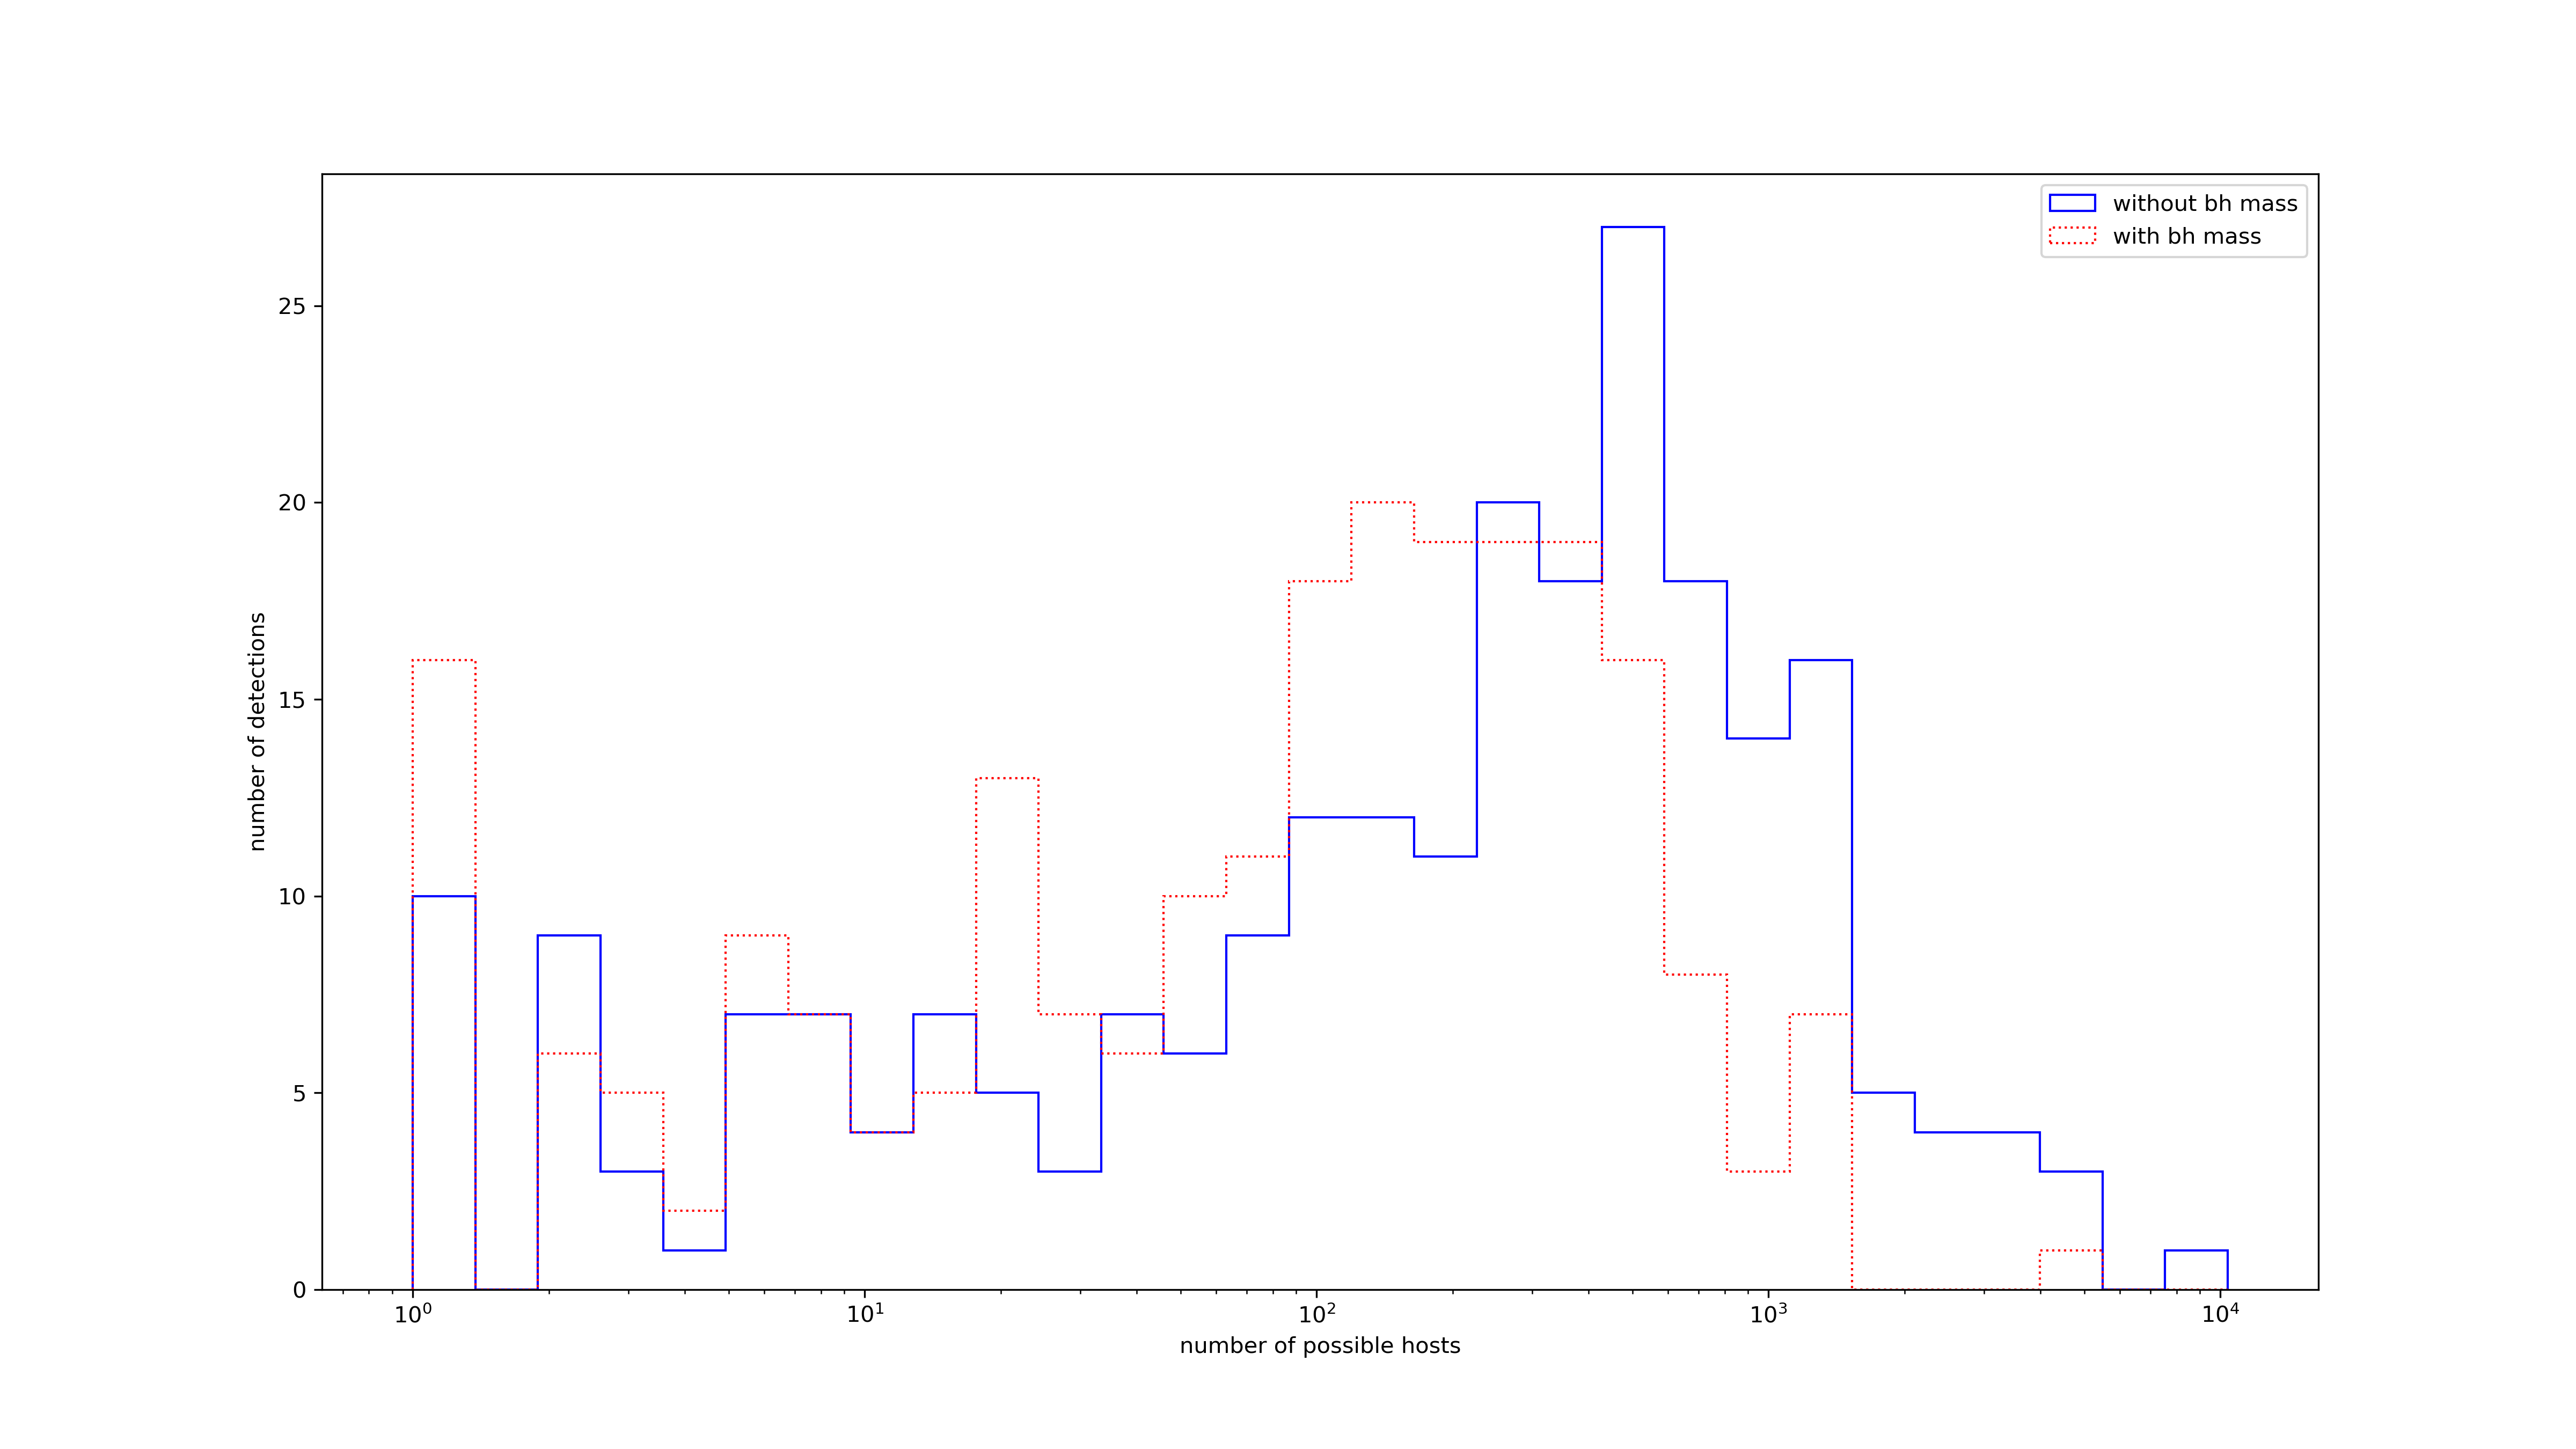
\includegraphics[width=0.8\textwidth]{number_of_possible_hosts.png}
    \caption[Number of possible hosts]{Number of possible hosts for each detection using a $3\sigma$ region on the considered parameters.}
    \label{fig:possible-hosts}
\end{figure}

\begin{figure}
    \centering
    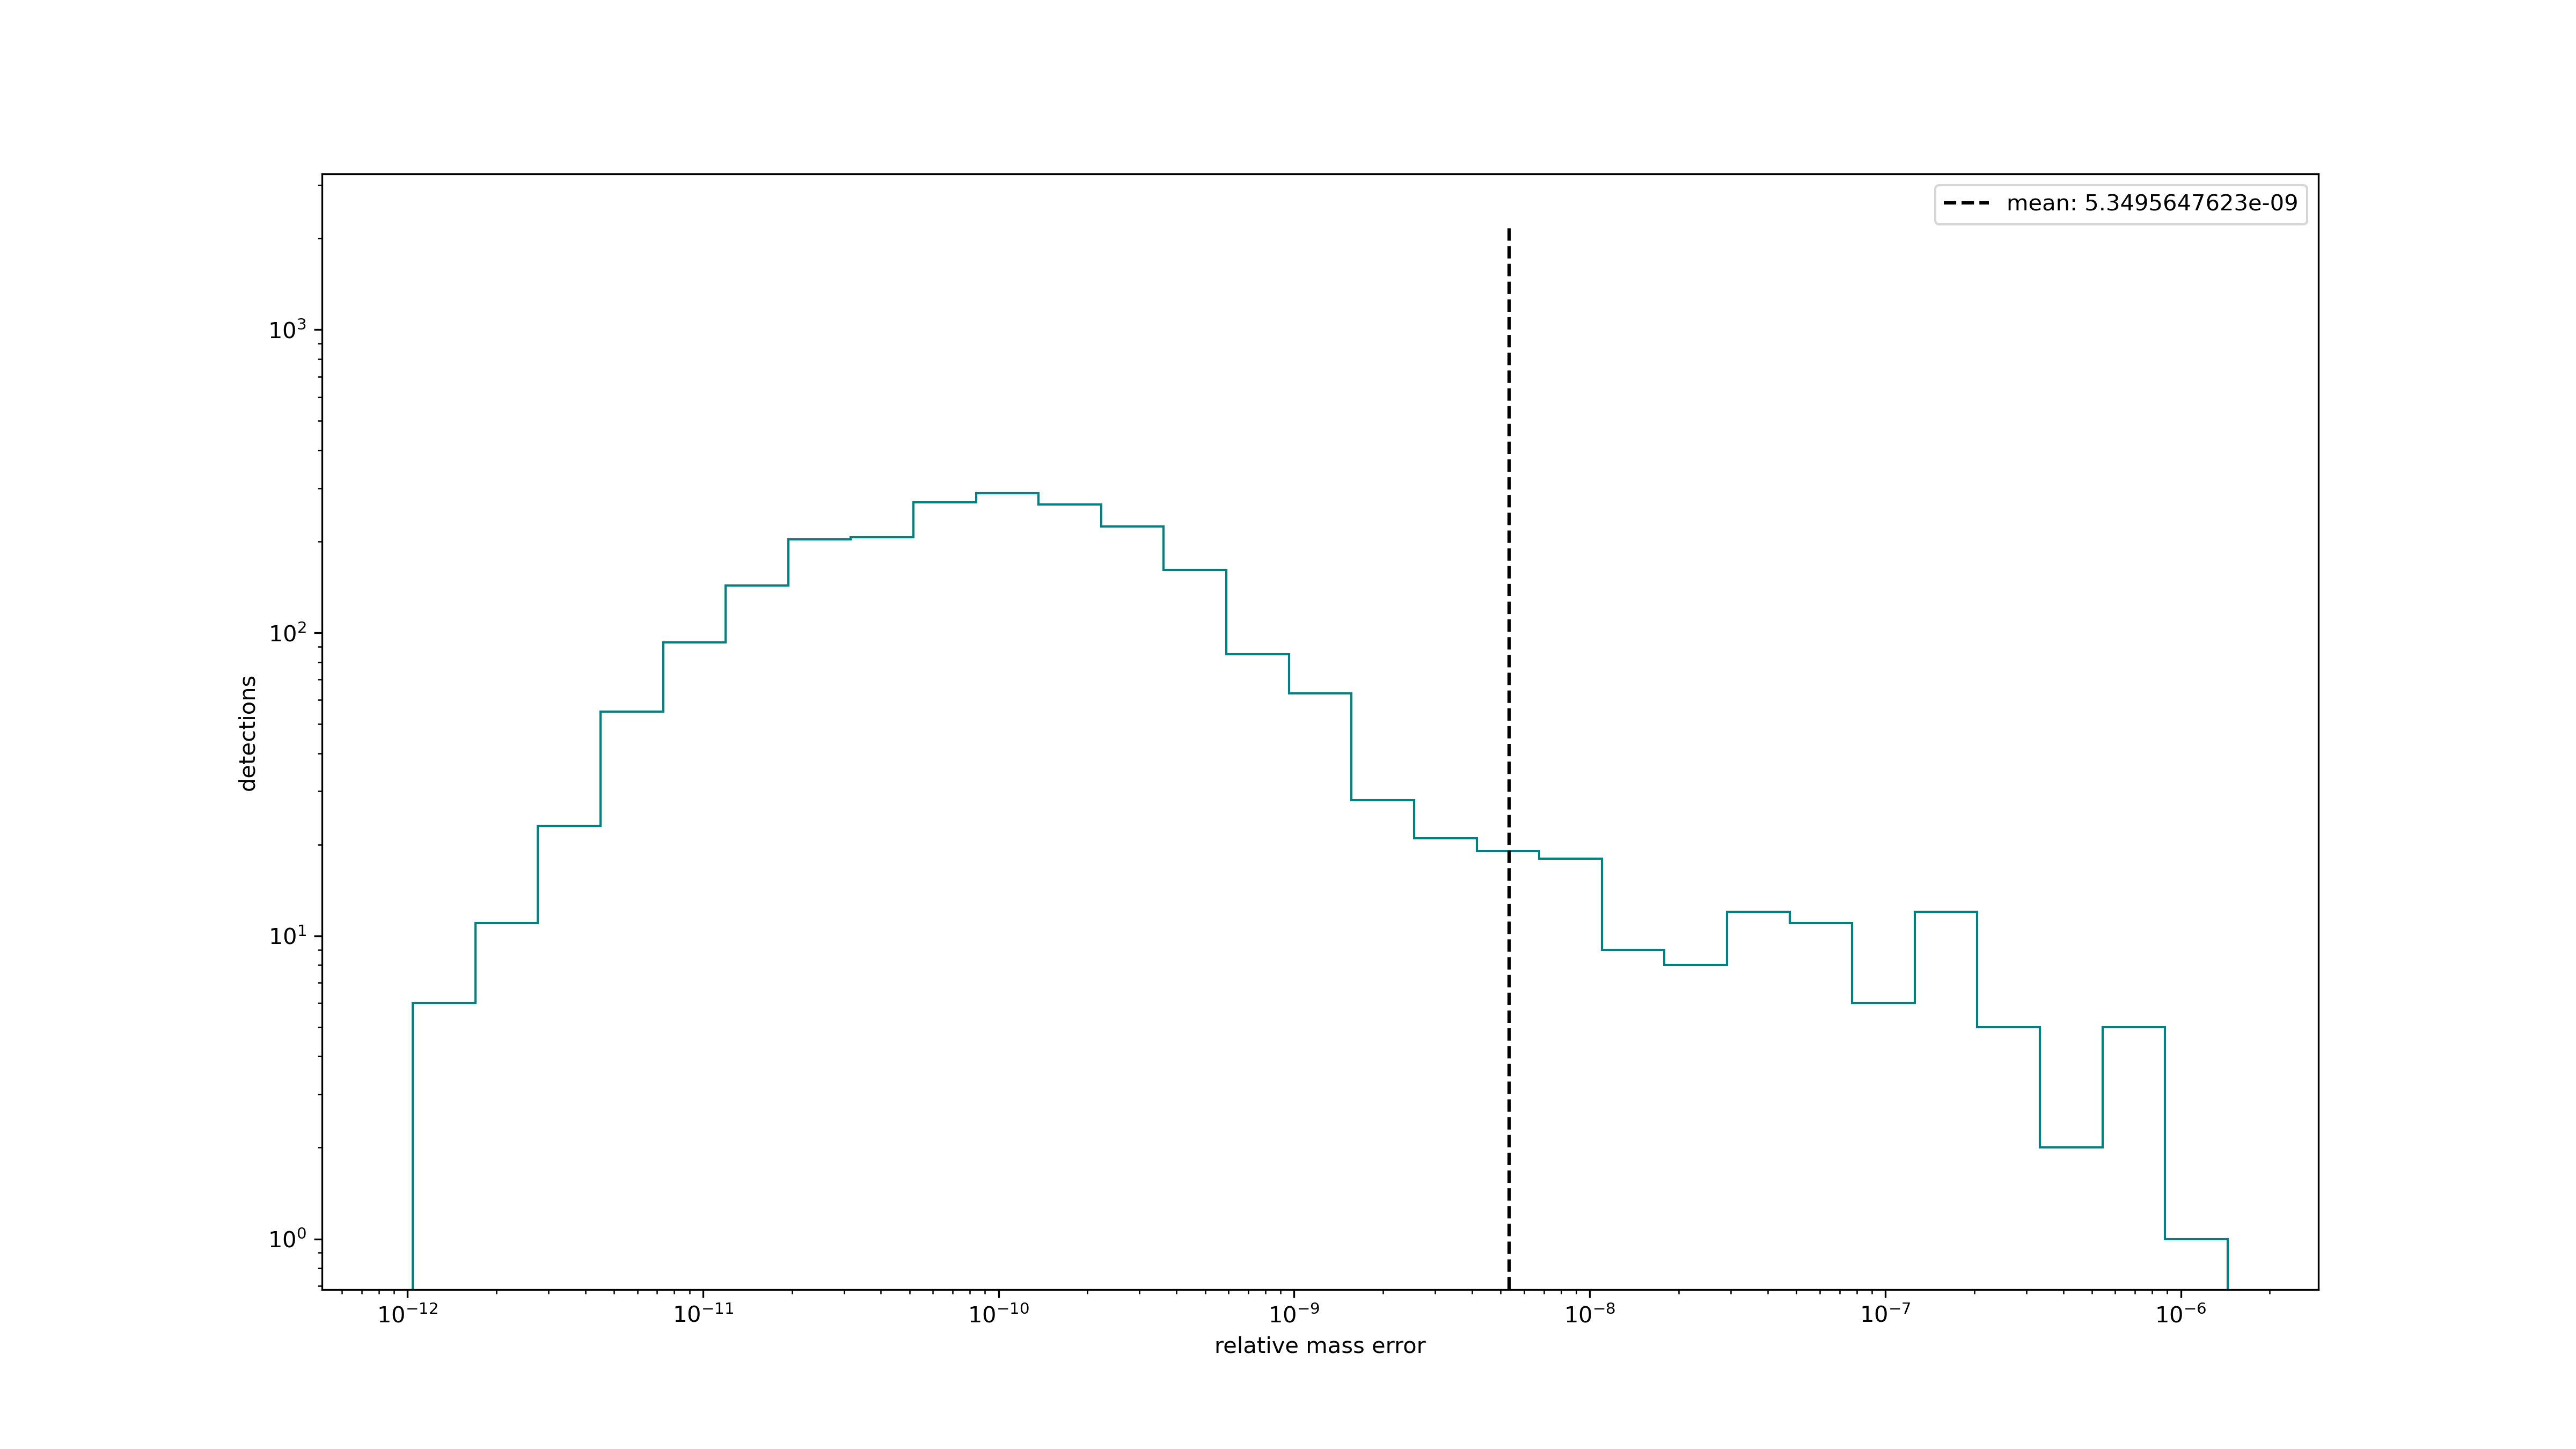
\includegraphics[width=0.49\textwidth]{relative_mass_error.png}
    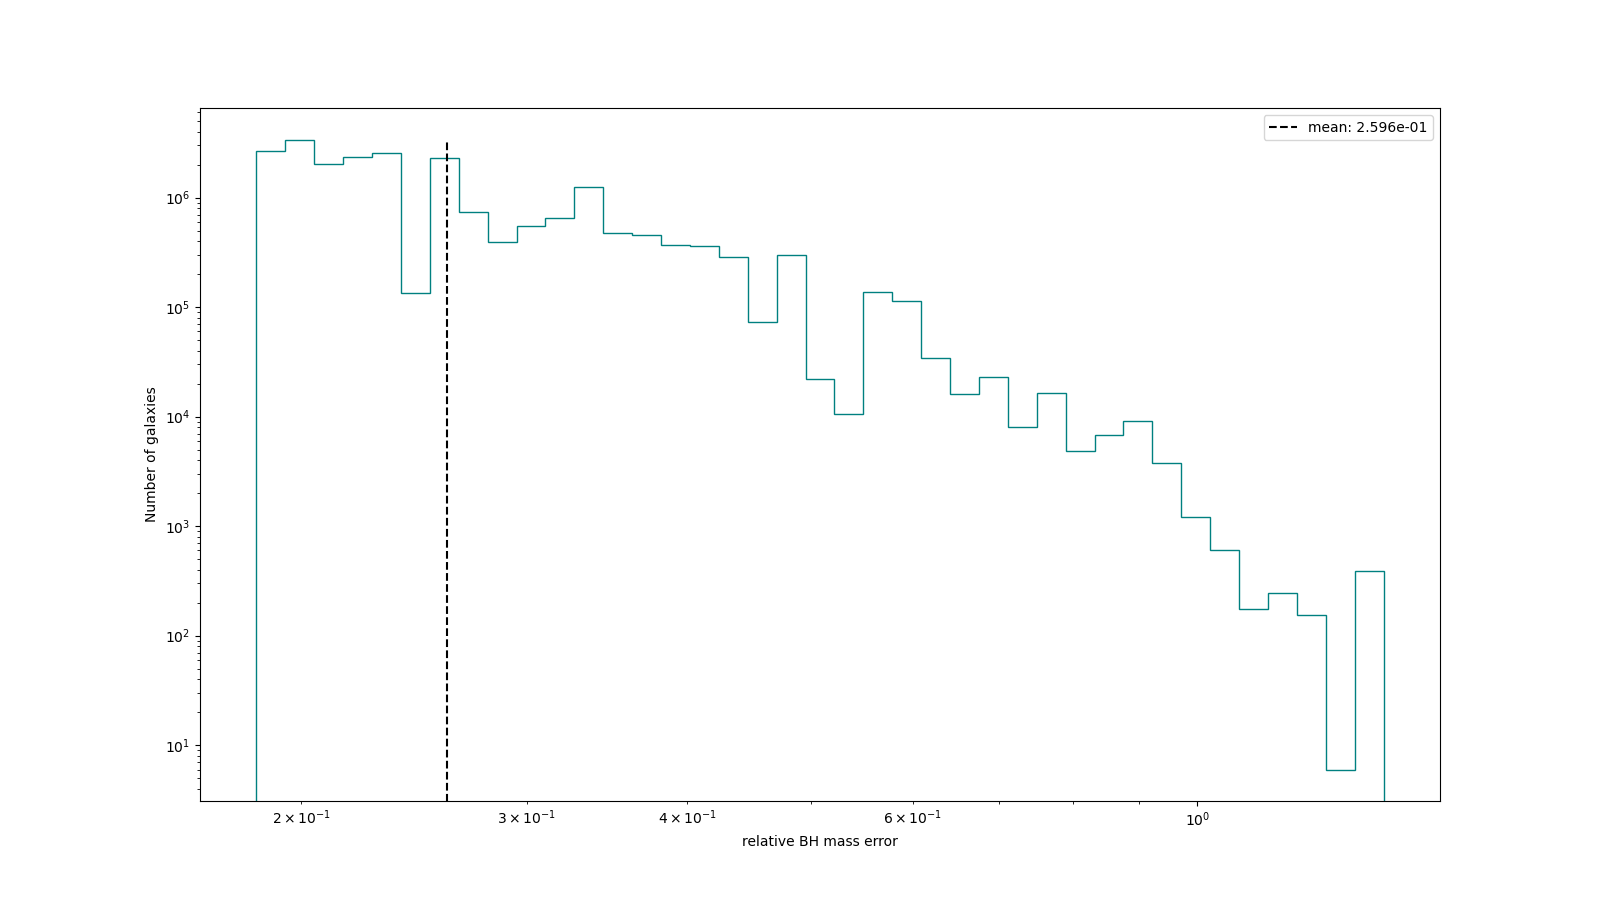
\includegraphics[width=0.49\textwidth]{relative_BH_mass_error_distribution.png}
    \caption[Relative mass error detection and galaxy catalog]{Left: relative mass error histogram for detections used in \fullref{ch:galaxy-catalog-as-ground-truth}. Right: relative mass error distribution for the galaxy catalog.}
    \label{fig:relative-mass-error-distribution}
\end{figure}


